\documentclass[letterpaper,11pt]{article}
\usepackage[spanish]{babel}
\usepackage{graphicx}
\usepackage{url}
\usepackage[utf8]{inputenc}
\usepackage{listings}
\usepackage{longtable}
\usepackage[small,bf]{caption}
\setlength{\parindent}{1em}

\begin{document}

\begin{figure}[htp]
  \centering
  
\includegraphics[scale=0.1]{logoUSB.png}
\end{figure}

\begin{center}
  \textbf{UNIVERSIDAD SIM\'ON BOL\'IVAR}\\
  Ingenier\'ia de la Computaci\'on\\
  Dise\~no de Algoritmos I - CI-5651
\end{center}
\begin{center}	
  \vspace{2in}
  \textsf{\begin{Large}\bf Implementaci\'on de un SAT-Solver para la resoluci\'on 
de instancias SAT de sudoku \\ \end{Large}}
      
\end{center}
\begin{center}
  \vspace{2in}
  Federico Flaviani 99-31744\\
  Sim\'on Rojas 03-36440\\
  Juan Garc\'ia 05-38207\\
  \vspace{0.25in}	
  \today
\end{center}
\newpage

\tableofcontents

\newpage
\setlength{\parskip}{8pt}. 
\section{Introducci\'on}
\emph{Sudoku} es un juego originario de Jap\'on que tiene como objetivo 
rellenar una cuadr\'icula de 9 x 9 celdas (81 casillas) divid\'ida en 
subcuadr\'iculas de 3 x 3 (tambi\'en llamadas ``cajas'' o ``regiones'') 
con las cifras del 1 al 9 partiendo de algunos n\'umeros ya dispuestos 
en algunas de las celdas. La idea es que no se debe repetir ninguna cifra en una 
misma fila, columna o subcuadr\'icula. Un sudoku est\'a bien planteado si la 
soluci\'on es \'unica.
\begin{figure}[htp]
  \centering
  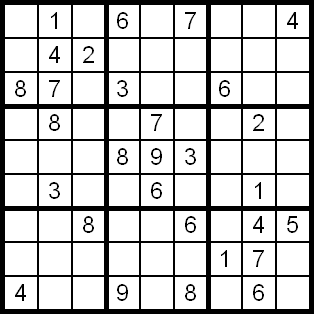
\includegraphics[scale=0.3]{sudoku.png}
  \caption{Ejemplo de un tablero de \emph{Sudoku}}
\end{figure}

\subsection{Motivaci\'on del proyecto}
A partir del an\'alisis de complejidad de algunos algoritmos, espec\'ificamente de 
aquellos que entran en el cunjunto de los NP (Nondeterministic Polynomial time), 
nos encontramos con el problema del sudoku general, un problema categorizado como 
NP-Hard, en donde hallar una soluci\'on se resume a realizar busquedas profundas 
dentro del ambiente de estados posibles.

Tomando como base el problema, la idea general es aplicar nuevos m\'etodos que 
permitan hallar la soluci\'on de una manera mas eficiente. Hasta ahora el mejor 
metodo que se puede usar es el \emph{Backtracking simple}, pero dentro de la gama 
de mejoras se pueden mencionar las t\'ecnicas de \emph{Backtraking no cronol\'ogico} 
y espec\'ificamente, para esta primera entrega, la implementaci\'on del 
\emph{Unit Propagation}.

\subsection{Breve descripci\'on del problema}
Dada una instancia de Sudoku con solo asignaciones parciales, se plantea buscar 
una soluci\'on, o lo que es igual, hallar el conjunto de asignaciones que deban 
realizarse para rellenar el tablero, y que satisfagan las condiciones de sudoku. 
Estas condiciones son las siguientes:
\begin{description}
\item[-] Cada celda debe contener un n\'umero del 1 al 9.
\item[-] Una celda no puede tener dos n\'umeros distintos.
\item[-] Dos casillas distintas en una misma fila, columna o subcuadr\'icula no 
puede contener el mismo n\'umero.
\end{description}
Para representar estas condiciones usaremos la \emph{Forma Normal Conjuntiva (CNF)}, 
en donde la f\'ormula del problema se plantea como una conjunci\'on de disjunciones, 
y el objetivo es encontrar el conjunto de asignaciones a las variables que mantengan
la condici\'on de True en la f\'ormula.

\subsection{Descripci\'on del contenido del informe}
En el siguiente informe se dar\'a una breve explicaci\'on del dise\~no e 
implementaci\'on del sat-solver orientado a la resoluci\'on del sudoku. Basicamente 
se explicar\'an las estructuras de datos usadas para representar el problema y los 
algoritmos utilizados. Ademas presentar aquellos problemas encontrados durante el 
desarrollo, una breve rese\~na de los elementos implementados y detalles en cuanto 
a la operatividad del programa. En general estamos presentando una guia para 
entender la manera en que atacamos la idea y como generamos una soluci\'on razonable 
para el problema del Sudoku general. 
\newpage

\section{Dise\~no}

\subsection{Modelo utilizado para representar el problema}
El modelo general para la resoluci\'on del problema del \emph{Sudoku} se basa en
tres partes. Un proceso de traducci\'on del problema a representaci\'on
SAT, siguiendo las restricciones que nos dieron en las reglas de resoluci\'on de juego. Luego la
busqueda de la soluci\'on mediante el sat-solver, el cual recibe la traducci\'on antes
realizada. Y por \'ultimo tomar la salida del solver y convertirla en una soluci\'on sudoku
mas legible.
La representaci\'on SAT se realiz\'o usando la forma normal conjuntiva (CNF), en donde
cada cl\'ausula que restringe el problema es presentada como una disjuncion de literales, 
y la formula total es una conjuncion de cl\'ausulas. Los literales no son mas que asignaciones 
True o False de variables en forma positiva (i) o negativa (-i).
Nuestra implementaci\'on tendra 4 m\'odulos, donde se destacan, un m\'odulo de traducci\'on 
del problema, uno de Listas auxiliares a usar en el algoritmo del solver, otro m\'odulo
que implementa directamente los algoritmos y por \'ultimo un m\'odulo de gerencia que
permite correr las diferentes herramientas con una sola ejecuci\'on.

\subsection{ Estructuras y algoritmos involucrados en la aplicaci\'on}
A continuaci\'on se explicaran las estruturas y algoritmos utilizado, lo dividiremos en
diferentes secciones, segun los m\'odulos explicados anteriormente:

\subsubsection{Traducci\'on}
El m\'odulo de traducci\'on se basa en leer las instancias parciales de sudoku, para luego 
representar mediante cl\'ausulas en CNF la representaci\'on SAT del problema general,
todo esto en conjunto con las asignaciones parciales realizadas. Todos los algoritmos utilizados
fueron simples iteraciones que iban escribiendo en el archivo de salida (``out.cnf''), las
cl\'ausulas necesarias segun las restricciones del problema.

\subsubsection{Herramientas Auxiliares}
En este modulo destaca la creaci\'on de una lista doblemente enlazada, que sera la estrucutura
que nos permitir\'a llevar un registro de literales y cl\'ausulas de una f\'ormula en CNF. B\'asicamente
se implement\'o el tipo abstracto Lista junto con una serie de operaciones elementales que trabajan
sobre el tipo para agregar, eliminar y recorrer elementos de la misma.

\subsubsection{SAT-Solver}
Para el SAT-solver fue necesario crear una serie de estructuras para representar de manera general
una f\'ormula normal conjuntiva. Se creo un arreglo para almacenar cada uno de los literales en memoria, y
los mismos se guardan en una estructura con diferentes campos, espec\'ificamente un 
campo que guarda el valor asignado y una lista de cl\'ausulas asociadas al literal.
Para representar una cl\'ausula se crea una estrucutra que guarda contadores sobre
los literales satisfechos o no satisfechos, asi como el tama\~no de una cl\'ausula,
una lista de literales contenidos y un literal que resguarda cuando una cl\'ausula es unitaria.
Para generalizar la f\'ormula, se crea una estructura que representa una f\'ormula
conjuntiva  y guarda el n\'umero de literales y cl\'ausulas totales, el arreglo de
literales, el numero de cl\'ausulas satisfechas y las variables asignadas.

\subsubsection{Soluci\'on}
Por \'ultimo tenemos el m\'odulo de soluci\'on, en donde se recibe la salida de los
respectivos solver y se procede a representar la soluci\'on obtenida en formato 
de sudoku general. Luego de esto se genera un archivo en formato Pdf que mostrar\'a la cuadr\'icula
con la soluci\'on de la instancia correspondiente.
\newpage

\section{Detalles de implementaci\'on}

\subsection{Rese\~na de los elementos implementados}
La estructura de datos que implementa la formula proposicional en forma 
normal conjuntiva viene dada por la siguiente estructura:

La f\'ormula consta de dos estructuras literales y Cl\'ausulas. 

\subsubsection{Objeto literal}
La implementaci\'on del objeto literal viene dado por un registro con dos 
campos: $valor$ y $clausulas$. El primero de ellos representa el valor de 
verdad del literal y el segundo es una lista de de las Cl\'ausulas que contienen 
a dicho literal

\subsubsection{Objeto Cl\'ausula}
La implementaci\'on del objeto Cl\'ausula viene dado por un registro con 
cinco campos: $satisfechos$, $noSatisfechos$, $tam$, $literales$ y 
$litUnitario$. $satisfechos$ y $noSatisfechos$ son enteros que determinan 
cuantos literales estan satisfechos o no en la Cl\'ausula en determinado 
momento. $tam$ es otro entero con el valor del n\'umero de literales de la 
Cl\'ausula. $literales$ es una lista que contienen todos los literales de 
la Cl\'ausula. $litUnitario$ es un apuntador que se\~nala a un literal, en 
el momento en que para una soluci\'on parcial \'este sea unitario.

\subsubsection{Objeto formula}
En un arreglo llamado literales colocamos los $2*|Var|$ posibles literales 
que existen sobre un conjunto de variables $Var$, en las posiciones 
dadas por la siguiente formula. 


$$literales[j]=\left\{\begin{array}{lcc}
              x_{(j/2)+1} & si & j~es~par \\
             \\ \overline{x_{(j+1)/2}}   & si & j~es~impar
             \end{array}
      \right.  $$

De esta forma $j$ identifica univocamente a cada literal, y por lo tanto 
basta saber el \'indice de alg\'un literal en particular, para ubicarlo dentro 
de una casilla del arreglo $literales$.

\subsection{Problemas encontrados}
\begin{itemize}
\item La extructura de datos que usamos nos permite saber si una clausula 
es unitaria facilmente. Sin embargo, no podemos saber con costo constante 
cual es el literal unitario de cada clausula unitaria, ya que tendriamos que 
recorrer toda la lista de literales para saberlo.

\item La selecci\'on de la pr\'oxima variable a ser evaluada la realizamos 
en orden lineal sobre sus identificadores. 
Tuvimos problemas para implementar unit propagation, debido a la falta 
de una extructura de datos, que nos permitiera selecionar cualquier variable 
distinta a este orden y que permitiera devolver la asignaci\'on a la hora 
del backtraking.

\item Se tuvo un problema en la utilizaci\'on del pure literal elimination durante el 
proceso de busqueda. Nosotros aplicamos esta tecnica solo como un 
preprocesamiento de la formula, antes de aplicar el algoritmo de DFS. 

Con la estructura de datos utilizada solo basta con verificar en el arreglo 
de literales, si existe una posici\'on cuyo literal tiene lista de clausulas 
vacia. Sin embargo, como nuestra estructura no elimina las clausulas que son 
satisfechas, durante las asignaciones parciales de variables, entonces en 
la corrida del DFS no van a existir mas listas (de clausulas) vacias de la 
que exist\'ian al principio, y por lo tanto no podemos ubicar literales 
puros con esta t\'ecnica (durante la busqueda).
\end{itemize}
\newpage

\section{Instrucciones de operaci\'on}
La aplicaci\'on tiene un script escrito en Python que llama al compilador para 
generar los distintos ejecutables. Luego procede a corre el traductor para
representar la instancia dada en formato SAT, y luego llamar a los respectivos
solvers para la resoluci\'on del problema. Al obtener la soluci\'on, procede a
generar los respectivos archivos en .pdf.
Con respecto a paquetes o librerias especiales solo se necesita lo siguiente:
\begin{description}
\item[-] Compilador Gcc para los programas escritos en C
\item[-] Libreria para correr programas en Python
\item[-] Libreria PdfLatex para generar los tableros
\end{description}
La \'unica linea que debera correr es la siguiente:
\begin{verbatim}
    $> python satSolver.py
\end{verbatim}
De igual manera se puede compilar y correr por separados el traductor y el solver. 

Para compilar el traductor solo debe realizar la llamada:
\begin{verbatim}
    $> make translator
\end{verbatim}
Para realizar la corrida:
\begin{verbatim}
    $> ./translator N_InstanciaParcial out.cnf
\end{verbatim}
El segundo argumento es una isntancia parcial del sudoku, en donde el primer 
numero N es el tama\~no del sudoku, luego un underscore (\_) y seguido la Instancia con
asignaci\'on parcial. En este caso, el traductor solo entrega la representaci\'on en CNF para la primera
instancia del archivo InstanciasSudoku.txt. De querer traducir todas, debe correr
el script en Python mencionado anteriormente.

Para compilar el solver debe llamar:
\begin{verbatim}
    $> make solver
\end{verbatim}
Y para correr el programa:
\begin{verbatim}
    $> ./solver out.cnf
\end{verbatim}
Donde out.cnf es la traducci\'on del problema de Sudoku a SAT.

Para compilar el solver de ZChaff:
\begin{verbatim}
    $> cd zchaff64/
    /zchaff64 $> make 
\end{verbatim}
\newpage

\section{Estado actual}

\subsection{Estado final de la aplicaci\'on}
El estado final de la aplicaci\'on no es operativo, espec\'ificamente en el m\'odulo del solver.
El traductor realiza su funci\'on perfectamente, tomando del archivo las instancias de sudoku
y entregando la traducci\'on a CNF. De igual manera el m\'odulo de soluci\'on, en donde se toma
la salida de los solvers y se entrega en formato sudoku pdf tambi\'en funciona.
El solver solo esta funcional para problemas SAT peque\~nos, al insertar un problema
de sudoku no logra finalizar. 
\subsection{Errores}
Dada la problem\'atica que tuvimos con la implementaci\'on del algoritmo DPLL, aunque el mismo logra
recorrer el arbol de posibles soluciones, dado que no se le pudo agregar el algoritmo de Unit
Propagation, esto repercute en que la resoluci\'on del problema del sudoku tarde mucho tiempo recorriendo
el arbol entero.
La problem\'atica encontrada con la implementaci\'on del DPLL es que las estructuras usadas y las
funciones de asignaci\'on de variables y actualizaci\'on de clausulas, complican la implementaci\'on del
unit propagation.
\newpage

\section{Conclusiones y recomendaciones}
Dado que no fue posible cumplir los objetivos planteados en el problema, son pocas las conclusiones
que podemos sacar. No pudimos obtener los tiempos comparativos entre los dos solvers, sin embargo se 
destaca el excelente rendimiento que tiene el solver Zchaff, el que resuelve todas las instancias en centesimas
de segundo, frente a nuestro solver propio que no consigue dar una soluci\'on en tiempo considerable.
En general encontramos una serie de problemas para implementar una buena soluci\'on al problema, mas que todo
por el enfoque que dimos a nivel de programaci\'on de los algoritmos. Por lo tanto resulta de vital importancia
plantear una soluci\'on mas eficiente y concisa de las funciones que se vayan a implementar para desarrollar
el solver.
\subsection{Mejoras}
\begin{itemize}
\item La estructura de datos usada para representar la formula en forma normal 
conjuntiva no es del tipo Lazy, en el sentido de que cuando sabemos que una 
clausula es satisfecha no la eliminamos de la lista de clausulas.

De esta forma en cada etapa de la busqueda la estructura no disminuye 
de tama\~no y en cada asignaci\'on de variable se deben recorrer listas de clausulas 
potencialmente grandes.

Sugerimos hacer las mejoras adecuadas para que nuestra estructura de datos que 
representa la formula proposicional, sea una estructura lazy.

\item Sugerimos incluir la rutina de pureLiteralElimination dentro del 
algoritmo de busqueda y no como un preprocesamiento de la f\'omula. Para 
que nuestra rutina pureLiteralElimination funcione durante el proceso de busqueda 
es necesario hacer la mejora descrita en el item anterior.

\item Nuestro algoritmo de busqueda en profundidad, es un algoritmo recursivo. 
Sugerimos reimplementar una versi\'on iterativa, para as\'i poder manejar 
con mayor facilidad la implementaci\'on de backtraking no cronol\'ogico.
\end{itemize}

\newpage

\section{Referencias bibliogr\'aficas}
\begin{thebibliography}{99}
  
\bibitem[1]{ref:data struct}
  \textbf{Efficient Data Structures for Fast SAT Solvers}\\
  \textit{LYNCE I., MARQUES-SILVA J.}

\bibitem[2]{ref:sat format}
  \textbf{Satisfiability Suggested Format}\\

\bibitem[3]{ref:sudoku as sat}
  \textbf{Sudoku as SAT Problem}\\
  \textit{LYNCE I., OUAKNINE J.}

\bibitem[4]{ref:ins sat}
  \textbf{url{http://www.cs.ubc.ca/$~$hoos/SATLIB/Benchmarks/SAT/satformat.ps}}
  
\end{thebibliography}
  
\end{document}
